%
% einleitung.tex -- Beispiel-File für die Einleitung
%
% (c) 2020 Prof Dr Andreas Müller, Hochschule Rapperswil
%
% !TEX root = ../../buch.tex
% !TEX encoding = UTF-8
%
\section{Vorwort\label{wavelets:section:teil0}}
\rhead{Vorwort}
Das Ziel dieser Arbeit war kein klares Ziel zu haben und zu schauen,
wo hin es einen trägt.
Natürlich war es notwendig sich einen Rahmen zu stecken, d.~h.~
eine grobe Wunschvorstellung festzulegen.
Aber tatsächlich war der Weg in dieser Arbeit das Ziel.
Die Wunschvorstellung war ein tieferes Verständnis über die
Wavelettransformation zu erhalten.
Hier muss angemerkt sein, dass es grundsätzlich zwei Oberbegriffe
im Zusammenhang mit Wavelets gibt.
Es kann einerseits eine diskrete und andererseits eine kontinuierliche
Wavelettransformation gemacht werden.

\begin{itemize}
\item   Die diskrete Wavelettransformation (DWT) arbeitet auf Basis
einer Filterbank, dient also dazu Signale direkt zu Filtern
z.~B.~rauschbelastete Signale zu Entrauschen.
\index{DWT}%
\index{diskrete Wavelettransformation}%
Die Funktionsweise kann man einfach als eine wiederholte
Aufsplittung in einen Tief- und Hochpass gefilterten
Signalteil beschreiben.
Wobei der Tiefpass jeweils den Durchschnitt über die Filterbreite
und der Hochpass die Änderung über die gefilterte Signalbreite
ausgibt (man spricht oft auch von der Detaillierung).
Für eine Entrauschung wird also eine Filterbank aufgebaut die gerade
\index{Filterbank}%
eine so hohe Detaillierung besitzt, dass die Rauschanteile eliminiert
werden (Abbildung \ref{wavelet:fig:1_Four-Level-Wavelet-Decomposition}).

\item Die kontinuierliche Wavelettransformation (CWT) ist
\index{CWT}%
\index{kontinuierliche Wavelettransformation}
die Transformation des Zeitsignals in den Frequenzbereich.
Der Ablauf ist relativ analog zur diskreten Fourier-Transformation
(DFT), wo die Unterschiede liegen und was die Vor- sowie die Nachteile
der CWT gegenüber der schnellen Fourier-Transformation (FFT) sind,
ist eines der Ziele dieser Arbeit.
\end{itemize}

\begin{figure}
	\centering
	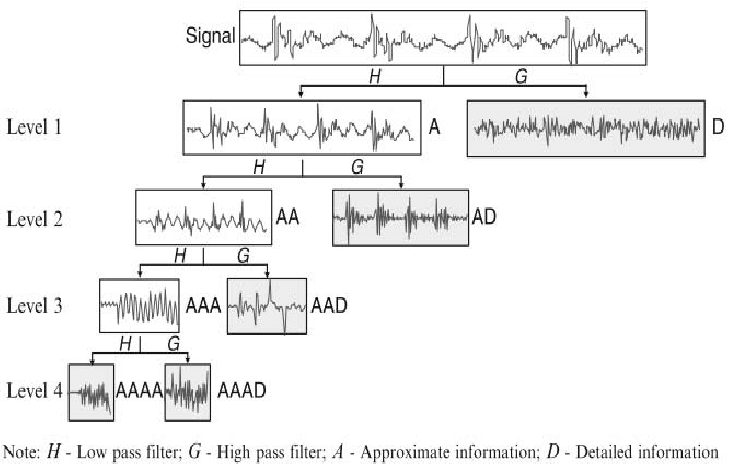
\includegraphics[width=0.75\textwidth]{papers/wavelets/images/1_Four-Level-Wavelet-Decomposition.png}
	\caption{\cite{wavelets:Haider.2015} Funktionsweise der diskreten Wavelettransformation (DWT).}
	\label{wavelet:fig:1_Four-Level-Wavelet-Decomposition}
\end{figure}

Die Untersuchung beschränkt sich aus zeitlichen Gründen auf die CWT.
Natürlich könnte man sich nun fertigen Tools bedienen und eine
Vielzahl von Spielereien damit durchführen.
Das Ziel ist aber nicht breit gefächert alle möglichen Tools
anzuwenden, vielmehr soll Verständnis für eine angewandte Transformation
aufgebaut werden.
Aus diesem Grund wird versucht, selbst ein lauffähiges CWT-Programm
zur Signalanalyse zu schreiben.

